\let\lesson\undefined
\newcommand{\lesson}{\phantomlesson{Bài 6.}}
\section{Bài tập trắc nghiệm}
\begin{enumerate}[label=\bfseries Câu \arabic*:, leftmargin=1.7cm]
	\item\mkstar{1}\\
	Hệ thức nào sau đây \textbf{không phù hợp} với quá trình đẳng áp?
	\begin{mcq}(4)
		\item $\dfrac{V}{T}=\text{const}$.
		\item $V\sim\dfrac{1}{T}$.
		\item $V\sim T$.
		\item $\dfrac{V_1}{T_1}=\dfrac{V_2}{T_2}$.
	\end{mcq}
\hideall{
\textbf{Đáp án B.}
}

\item \mkstar{1}\\
Một thí nghiệm được thực hiện với khối không khí chứa trong bình cầu 
và ngăn với khí quyển bằng giọt thủy ngân như hình vẽ. Khi làm nóng hay nguội  bình cầu thì biến đổi của khối khí thuộc loại nào?
\begin{center}
	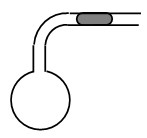
\includegraphics[width=0.15\linewidth]{../figs/VN12-Y24-PH-SYL-011P-3}
\end{center}
\begin{mcq}(4)
	\item Đẳng áp.
	\item Đẳng tích.
	\item Đẳng nhiệt.
	\item Bất kì.
\end{mcq}
\hideall{
\textbf{Đáp án A.}
}


\item \mkstar{1}\\
Trong hệ toạ độ $OVT$, đường biểu diễn nào sau đây là đường đẳng áp?
\begin{mcq}(2)
	\item Đường thẳng song song với trục hoành.
	\item Đường thẳng song song với trục tung.
	\item Đường hyperbol.
	\item Đường thẳng kéo dài đi qua gốc toạ độ.
\end{mcq}
\hideall{
\textbf{Đáp án D.}
}

\item \mkstar{2}\\
Một quả bóng bay chứa khí hydrogen vào buổi sáng ở nhiệt độ $\SI{20}{\celsius}$ thì có thể tích $\SI{2500}{\centi\meter^3}$. Coi áp suất khí quyển trong ngày không đổi. Thể tích của quả bóng này vào buổi trưa có nhiệt độ $\SI{35}{\celsius}$ \textbf{gần nhất} với giá trị nào sau đây?
\begin{mcq}(4)
	\item $\SI{4375}{\centi\meter^3}$.
	\item $\SI{2628}{\centi\meter^3}$.
	\item $\SI{2378}{\centi\meter^3}$.
	\item $\SI{1429}{\centi\meter^3}$.
\end{mcq}
\hideall{
\textbf{Đáp án B.}\\
\begin{center}
	\begin{tabular}{C{4cm} C{3cm} C{4cm}}
		\colorbox{yellow}{\textcolor{red}{\textbf{Trạng thái 1}}} & $\xrightarrow[]{p_1=p_2}$ & \colorbox{yellow}{\textcolor{red}{\textbf{Trạng thái 2}}}\\
		$V_1=\SI{2500}{\centi\meter^3}$ & &$V_2=?$\\
		$T_1=\SI{293}{\kelvin}$ & & $T_2=\SI{308}{\kelvin}$
	\end{tabular}

\end{center}
$$\dfrac{V_1}{T_1}=\dfrac{V_2}{T_2}\Rightarrow V_2\approx\SI{2628}{\centi\meter^3}.$$
}

\item Ở nhiệt độ $\SI{273}{\celsius}$ thể tích của một khối khí lí tưởng là $\SI{10}{\liter}$. Trong điều kiện áp suất không đổi, thể tích của khối khí đó ở nhiệt độ $\SI{546}{\celsius}$ là
\begin{mcq}(4)
	\item $\SI{20}{\liter}$.
	\item $\SI{15}{\liter}$.
	\item $\SI{12}{\liter}$.
	\item $\SI{13.5}{\liter}$.
\end{mcq}
\hideall{
\begin{center}
	\begin{tabular}{C{4cm} C{3cm} C{4cm}}
		\colorbox{yellow}{\textcolor{red}{\textbf{Trạng thái 1}}} & $\xrightarrow[]{p_1=p_2}$ & \colorbox{yellow}{\textcolor{red}{\textbf{Trạng thái 2}}}\\
		$V_1=\SI{10}{\liter}$ & &$V_2=?$\\
		$T_1=\SI{546}{\kelvin}$ & & $T_2=\SI{819}{\kelvin}$
	\end{tabular}
\end{center}
$$\dfrac{V_1}{T_1}=\dfrac{V_2}{T_2}\Rightarrow V_2=\SI{15}{\liter}.$$
}

\item\mkstar{2}\\ 
Một khối khí lí tưởng ban đầu có các thông số trạng thái $p_0$; $V_0$; $T_0$. Khối khí biến đổi đẳng áp đến thể tích $2V_0$ rồi biến đổi đẳng nhiệt về thể tích ban đầu. Đồ thị nào sau đây diễn tả \textbf{đúng} quá trình trên?
\begin{center}
	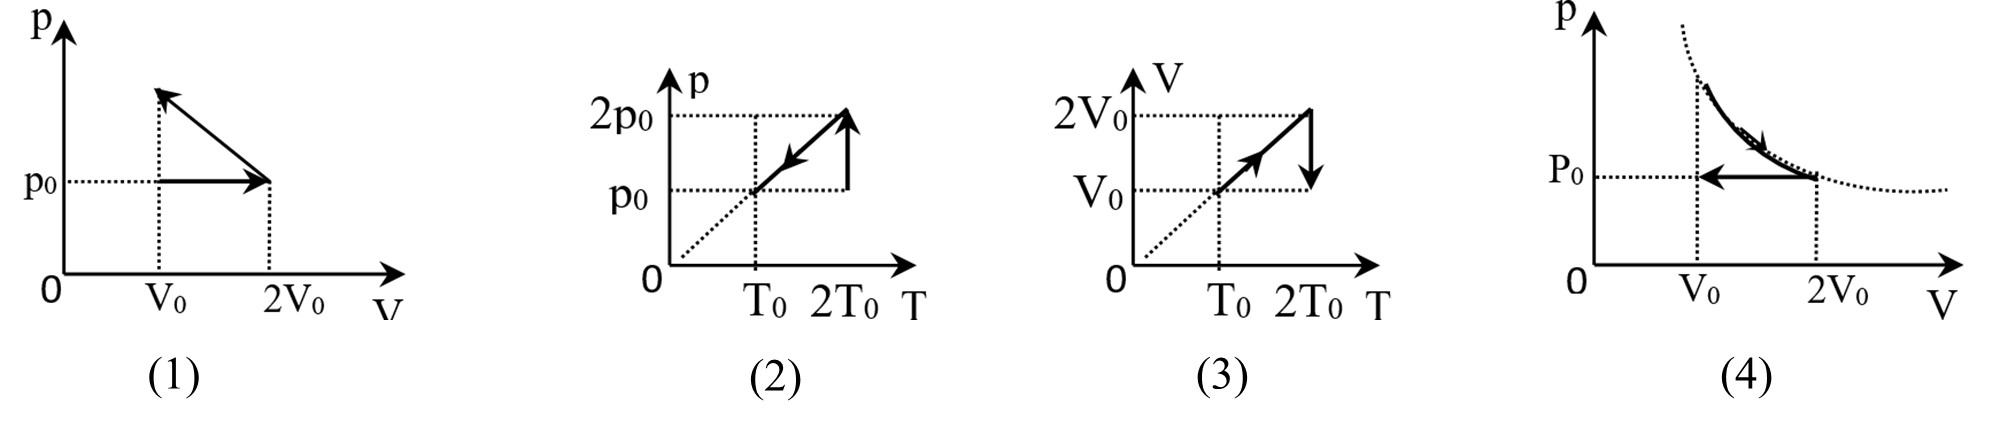
\includegraphics[width=0.9\linewidth]{../figs/VN12-Y24-PH-SYL-011P-4}
\end{center}
\begin{mcq}(4)
	\item (1).
	\item (2).
	\item (3).
	\item (4).
\end{mcq}
\hideall{
\textbf{Đáp án C.}
}

\item \mkstar{2}\\
Thể tích của một lượng khí xác định tăng thêm $\SI{10}{\percent}$  khi nhiệt độ của khí được tăng tới $\SI{47}{\celsius}$. Xác định nhiệt độ ban đầu của lượng khí, biết quá trình trên là đẳng áp.
\begin{mcq}(4)
	\item $\SI{18}{\celsius}$.
	\item $\SI{42}{\celsius}$.
	\item $\SI{51.7}{\celsius}$.
	\item $\SI{79}{\celsius}$.
\end{mcq}
\hideall{
\textbf{Đáp án A.}\\
$$\dfrac{T_1}{T_2}=\dfrac{V_1}{V_2}\Rightarrow T_1=\dfrac{T_2}{1,1}\approx\SI{291}{\kelvin}\Rightarrow t_1=\SI{18}{\celsius}.$$
}

\item \mkstar{2}\\
Một khối khí có thể tích $\SI{10}{\liter}$ ở $\SI{27}{\celsius}$. Giữ cho áp suất của khối khí không thay đổi, phải tăng nhiệt độ của khối khí lên bao nhiêu độ nữa để thể tích của nó là $\SI{12}{\liter}$?
\begin{mcq}(4)
	\item $\SI{300}{\kelvin}$.
	\item $\SI{360}{\kelvin}$.
	\item $\SI{60}{\kelvin}$.
	\item $\SI{120}{\kelvin}$.
\end{mcq}
\hideall{
\textbf{Đáp án C.}\\
\begin{center}
	\begin{tabular}{C{4cm} C{3cm} C{4cm}}
		\colorbox{yellow}{\textcolor{red}{\textbf{Trạng thái 1}}} & $\xrightarrow[]{p_1=p_2}$ & \colorbox{yellow}{\textcolor{red}{\textbf{Trạng thái 2}}}\\
		$V_1=\SI{10}{\liter}$ & &$V_2=\SI{12}{\liter}$\\
		$T_1=\SI{300}{\kelvin}$ & & $T_2=?$
	\end{tabular}
\end{center}
	$$\dfrac{V_1}{T_1}=\dfrac{V_2}{T_2}\Rightarrow T_2=\SI{360}{\kelvin}\Rightarrow \Delta T=\SI{60}{\kelvin}.$$
}

\item \mkstar{2}\\
Khi nhiệt độ của khối khí lí tưởng tăng từ $\SI{27}{\celsius}$ đến $\SI{227}{\celsius}$ đồng thời giữ khối lượng và áp suất khí không đổi thì thể tích của khí sẽ
\begin{mcq}(4)
	\item tăng lên $\SI{66.67}{\percent}$.
	\item giảm xuống $\SI{66.67}{\percent}$.
	\item tăng lên $\SI{40}{\percent}$.
	\item giảm xuống $\SI{40}{\percent}$.
\end{mcq}
\hideall{
\textbf{Đáp án A.}\\
$$\dfrac{V_2}{V_1}=\dfrac{T_2}{T_1}=\dfrac{5}{3}\approx\SI{166.67}{\percent}.$$
}

\item \mkstar{2}\\
Một khối khí $\SI{12}{\gram}$ có thể tích $\SI{4}{\liter}$ ở nhiệt độ $\SI{7}{\celsius}$. Sau khi được đun nóng đẳng áp thì khối lượng riêng của khí là $\SI{1.2}{\gram/\liter}$. Nhiệt độ của khí sau khi được đun nóng là
\begin{mcq}(4)
	\item $\SI{84}{\celsius}$.
	\item $\SI{574}{\celsius}$.
	\item $\SI{247}{\celsius}$.
	\item $\SI{427}{\celsius}$.
\end{mcq}
\hideall{
\textbf{Đáp án D.}\\
\begin{center}
	\begin{tabular}{C{4cm} C{3cm} C{4cm}}
		\colorbox{yellow}{\textcolor{red}{\textbf{Trạng thái 1}}} & $\xrightarrow[]{p_1=p_2}$ & \colorbox{yellow}{\textcolor{red}{\textbf{Trạng thái 2}}}\\
		$V_1=\SI{4}{\liter}$ & &$V_2=\SI{10}{\liter}$\\
		$T_1=\SI{280}{\kelvin}$ & & $T_2=?$
	\end{tabular}
\end{center}
}

\item \mkstar{2}\\
Nung nóng một lượng khí trong điều kiện đẳng áp, người ta thấy  khi nhiệt độ của khối khí tăng thêm $\SI{3}{\kelvin}$ thì thể tích tăng thêm $\SI{1}{\percent}$ so với thể tích ban đầu. Nhiệt độ ban đầu của lượng khí trên là
\begin{mcq}(4)
	\item $\SI{17}{\celsius}$.
	\item $\SI{56}{\celsius}$.
	\item $\SI{27}{\celsius}$.
	\item $\SI{36}{\celsius}$.
\end{mcq}
\hideall{
\textbf{Đáp án C.}\\
\begin{center}
	\begin{tabular}{C{4cm} C{3cm} C{4cm}}
		\colorbox{yellow}{\textcolor{red}{\textbf{Trạng thái 1}}} & $\xrightarrow[]{p_1=p_2}$ & \colorbox{yellow}{\textcolor{red}{\textbf{Trạng thái 2}}}\\
		$V_1$ & &$V_2=1,01V_1$\\
		$T_1=?$ & & $T_2=T_1+3$
	\end{tabular}
\end{center}
Theo định luật Charles:
$$\dfrac{T_1}{V_1}=\dfrac{T_1+3}{1,01V_1}\Rightarrow T_1=\SI{300}{\kelvin}\Rightarrow t_1=\SI{27}{\celsius}.$$
}

\item \mkstar{3}\\
Ống thuỷ tinh tiết diện đều với một đầu kín và một đầu hở. Bên trong ống có cột không khí dài $\ell_1=\SI{20}{\centi\meter}$ được ngăn cách với không khí bên ngoài bởi cột thuỷ ngân, nhiệt độ bên trong ống là $\SI{27}{\celsius}$. Khi nhiệt độ không khí bên trong ống tăng thêm $\SI{10}{\celsius}$ thì chiều cao cột không khí bên trong ống là bao nhiêu nếu áp suất của khí không đổi?
\begin{mcq}(4)
	\item $\SI{22}{\centi\meter}$.
	\item $\SI{19.68}{\centi\meter}$.
	\item $\SI{20.67}{\centi\meter}$.
	\item $\SI{18.96}{\centi\meter}$.
\end{mcq}
\hideall{\textbf{Đáp án C.}
\begin{center}
	\begin{tabular}{C{4cm} C{3cm} C{4cm}}
		\colorbox{yellow}{\textcolor{red}{\textbf{Trạng thái 1}}} & $\xrightarrow[]{p_1=p_2}$ & \colorbox{yellow}{\textcolor{red}{\textbf{Trạng thái 2}}}\\
		$V_1=\ell_1S$ & &$V_2=\ell_2S$\\
		$T_1=\SI{300}{\kelvin}$ & & $T_2=\SI{310}{\kelvin}$
	\end{tabular}
\end{center}
$$\dfrac{V_1}{T_1}=\dfrac{V_2}{T_2}\Rightarrow \ell_2\approx\SI{20.67}{\centi\meter}.$$
}

\item \mkstar{3}\\
Một bình dung tích $V=\SI{15}{\centi\meter^3}$ chứa không khí ở nhiệt độ $t_1=\SI{177}{\celsius}$ nối với một ống nằm ngang chứa đầy thuỷ ngân, đầu kia của ống thông với không khí bên ngoài. Khối lượng riêng của thuỷ ngân là $\SI{13.6}{\gram/\centi\meter^3}$. Khi nhiệt độ trong bình được làm lạnh đến nhiệt độ $t_2=\SI{27}{\celsius}$ thì khối lượng thuỷ ngân chảy vào bình là
\begin{mcq}(4)
	\item $\SI{5}{\gram}$.
	\item $\SI{172.88}{\gram}$.
	\item $\SI{68}{\gram}$.
	\item $\SI{136}{\gram}$.
\end{mcq}
\hideall{
\textbf{Đáp án C.}\\
\begin{center}
	\begin{tabular}{C{4cm} C{3cm} C{4cm}}
		\colorbox{yellow}{\textcolor{red}{\textbf{Trạng thái 1}}} & $\xrightarrow[]{p_1=p_2}$ & \colorbox{yellow}{\textcolor{red}{\textbf{Trạng thái 2}}}\\
		$V_1=\SI{15}{\centi\meter^3}$ & &$V_2=?$\\
		$T_1=\SI{450}{\kelvin}$ & & $T_2=\SI{300}{\kelvin}$
	\end{tabular}
\end{center}
$$\dfrac{V_1}{T_1}=\dfrac{V_2}{T_2}\Rightarrow V_2=\SI{10}{\centi\meter^3}.$$
Thể tích thuỷ ngân chảy vào bình là
$$\Delta V=V_2-V_1=\SI{5}{\centi\meter^3}.$$
Khối lượng thuỷ ngân chảy và bình là
$$\Delta m=\rho \Delta V=\SI{68}{\gram}.$$}

\item \mkstar{3}\\
Cho áp kế như hình vẽ. Ống thuỷ tinh dài có tiết diện $\SI{0.1}{\centi\meter^2}$. Ở $\SI{0}{\celsius}$ giọt thuỷ ngân cách A là $\SI{30}{\centi\meter}$, ở $\SI{5}{\celsius}$ giọt thuỷ ngân cách A là $\SI{50}{\centi\meter}$. Thể tích của bình là
\begin{center}
	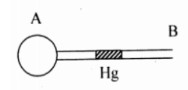
\includegraphics[width=0.3\linewidth]{../figs/VN12-Y24-PH-SYL-011P-2}
\end{center}
\begin{mcq}(4)
	\item $\SI{106}{\centi\meter^3}$.
	\item $\SI{210}{\centi\meter^3}$.
	\item $\SI{134}{\centi\meter^3}$.
	\item $\SI{250}{\centi\meter^3}$.
\end{mcq}
\hideall{
\textbf{Đáp án A.}\\
\begin{center}
	\begin{tabular}{C{4cm} C{3cm} C{4cm}}
		\colorbox{yellow}{\textcolor{red}{\textbf{Trạng thái 1}}} & $\xrightarrow[]{p_1=p_2}$ & \colorbox{yellow}{\textcolor{red}{\textbf{Trạng thái 2}}}\\
		$V_1=V+\SI{3}{\centi\meter^3}$ & &$V_2=V+\SI{5}{\centi\meter^3}$\\
		$T_1=\SI{273}{\kelvin}$ & & $T_2=\SI{278}{\kelvin}$
	\end{tabular}
\end{center}
$$\dfrac{V_1}{T_1}=\dfrac{V_2}{T_2}\Rightarrow V\approx\SI{106}{\centi\meter^3}.$$
}
\end{enumerate}
\section{Bài tập đúng/sai}
\begin{enumerate}[label=\bfseries Câu \arabic*:, leftmargin=1.7cm]
	\item \mkstar{2}\\
	Hiện nay, nồi áp suất là một trong các thiệt bị gia dụng được sử dùng phổ biến. Nồi áp suất giúp rút ngắn thời gian đun nấu, đa dạng chế độ nấu và an toàn cao nhờ hệ thống khoá nắp nồi khi chưa xả hết khí ra ngoài.
	\begin{center}
		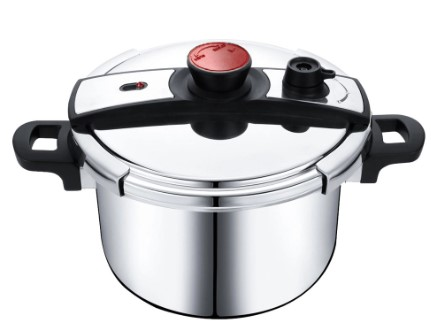
\includegraphics[width=0.\linewidth]{../figs/VN12-Y24-PH-SYL-011P-5}
	\end{center}
\begin{enumerate}[label=\alph*)]
	\item Trong quá trình đun, áp suất bên trong nồi cao hơn áp suất khí quyển.
	\item Quá trình đun nấu diễn ra nhanh hơn do nước trong nồi áp suất sôi ở nhiệt độ thấp hơn $\SI{100}{\celsius}$.
	\item Van xả khí giúp cho khí và hơi nước trong nồi được xả ra ngoài một cách từ từ đến khi cân bằng với áp suất bên ngoài.
	\item Nếu không có khoá an toàn và mở nắp nồi khi khí chưa được xả ra ngoài thì nước trong nồi sẽ nhanh chóng chuyển thành hơi đồng thời phun ra ngoài.
\end{enumerate}
\hideall{
\begin{enumerate}[label=\alph*)]
	\item Đúng.
	\item Sai.
	\item Đúng.
	\item Đúng.
\end{enumerate}
}
\end{enumerate}

\section{Bài tập tự luận}
\begin{enumerate}[label=\bfseries Câu \arabic*:, leftmargin=1.7cm]
	
	\item\mkstar{3}\\
	Khi tăng nhiệt độ của một lượng khí xác định từ $\SI{32}{\celsius}$ lên $\SI{117}{\celsius}$ và giữ áp suất không đổi thì thể tích khí tăng thêm $\SI{1.7}{\liter}$. Thể tích của lượng khí sau khi tăng nhiệt độ là bao nhiêu?
	\hideall{
	\begin{center}
		\begin{tabular}{C{4cm} C{3cm} C{4cm}}
			\colorbox{yellow}{\textcolor{red}{\textbf{Trạng thái 1}}} & $\xrightarrow[]{p_1=p_2}$ & \colorbox{yellow}{\textcolor{red}{\textbf{Trạng thái 2}}}\\
			$V_1=V_2-\SI{1.7}{\liter}$ & &$V_2=?$\\
			$T_1=\SI{305}{\kelvin}$ & & $T_2=\SI{390}{\kelvin}$
		\end{tabular}
	\end{center}
$$\dfrac{V_1}{T_1}=\dfrac{V_2}{T_2}\Rightarrow V_2=\SI{7.8}{\liter}.$$
}

\item \mkstar{2}\\
Khối lượng riêng không khí trong phòng ở nhiệt độ $\SI{27}{\celsius}$ lớn hơn khối lượng riêng của không khí ngoài sân nắng ở nhiệt độ $\SI{42}{\celsius}$ bao nhiêu lần. Biết áp suất không khí trong và ngoài phòng là như nhau.
\hideall{
$$\dfrac{D_1}{D_2}=\dfrac{V_2}{V_1}=\dfrac{T_2}{T_1}=1,05.$$
}

\item \mkstar{3}\\
Khí ở lò thoát ra theo ống khói hình trụ. Ở đầu dưới, khí có nhiệt độ $\SI{727}{\celsius}$ và chuyển động với tốc độ $\SI{5}{\meter/\second}$. Áp suất khí coi như không đổi. Ở đầu trên của ống, khí có nhiệt độ $\SI{227}{\celsius}$. Tốc độ của khí ở đầu trên bằng bao nhiêu?
\hideall{
	\begin{center}
\begin{tabular}{C{4cm} C{3cm} C{4cm}}
	\colorbox{yellow}{\textcolor{red}{\textbf{Trạng thái 1}}} & $\xrightarrow[]{p_1=p_2}$ & \colorbox{yellow}{\textcolor{red}{\textbf{Trạng thái 2}}}\\
	$V_1=v_1tS$ & &$V_2=v_2tS$\\
	$T_1=\SI{1000}{\kelvin}$ & & $T_2=\SI{500}{\kelvin}$
\end{tabular}
\end{center}
$$\dfrac{V_1}{T_1}=\dfrac{V_2}{T_2}\Rightarrow v_2=\SI{2.5}{\meter/\second}.$$
}
\end{enumerate}



